%% ----------------------------------------------------------------------
%% START OF FILE
%% ----------------------------------------------------------------------

\chapter{设计实现}
\label{cha:mainmatter}

\section{缓存算法通用接口}
\label{sec:cache_interface}

\subsection{数据结构}
\begin{itemize}

\item 缓存块(CACHE\_BLOCK)

记录SSD缓存块和HDD存储块,最小的Cache存储单元。
\begin{lstlisting}
typedef struct _CACHE_BLOCK
{
    ULONGLONG Index;        //存储块索引,标记对应的HDD块
    ULONGLONG StorageIndex; //Cache块索引,SSD数据块指针
    BOOLEAN   Modified;     //更改标志
}CACHE_BLOCK, *PCACHE_BLOCK;
\end{lstlisting}

\item 缓存池(CACHE\_POOL)
\\Cache存储块池,用于组织存储块,记录Cache池的使用情况。
\begin{lstlisting}
typedef struct _CACHE_POOL
{
    ULONG        Size;       //Cache池总大小
    ULONG        Used;       //Cache池已使用存储块数量
    STORAGE_POOL Storage;    //存储池,管理底层存储介质访问
    ULONG32      ReadCount;  //读计数
    ULONG32      WriteCount; //写计数
    ULONG32      ReadHit;    //读命中计数
    ULONG32      WriteHit;   //写命中计数
}CACHE_POOL, *PCACHE_POOL;
\end{lstlisting}

\end{itemize}

\subsection{外部函数接口}
\begin{itemize}

\item InitCachePool
\\初始化Cache存储块池。初始化成功返回TRUE,否则返回FALSE。
\begin{lstlisting}
bool InitCachePool (
    PCACHE_POOL CachePool
);
\end{lstlisting}

\item DestroyCachePool
\\销毁Cache存储块池,释放存储空间。
\begin{lstlisting}
void DestroyCachePool (PCACHE_POOL CachePool);
\end{lstlisting}

\item QueryAndCopyFromCachePool
\\查询Cache池中的数据是否命中以Offset开始,以长度为Length的HDD数据。如果完全命中,拷贝数据到Buffer,返回TRUE;如果不命中,返回FALSE。
\begin{lstlisting}
bool QueryAndCopyFromCachePool (
    PCACHE_POOL CachePool,
    PUCHAR Buf,
    LONGLONG Offset,
    ULONG Length
);
\end{lstlisting}

\item QueryAndWriteToCachePool
\\查询Cache池中的数据是否命中以Offset开始,以长度为Length的HDD数据。如果存在命中部分,使用Buf更新Cache池中的数据,返回TRUE;如果不命中,返回FALSE。
\begin{lstlisting}
bool QueryAndWriteToCachePool (
    PCACHE_POOL CachePool,
    PUCHAR Buf,
    LONGLONG Offset,
    ULONG Length
);
\end{lstlisting}

\item ReadUpdataCachePool
\\使用Cache替换算法,利用Buffer中的数据进行Cache池的更新。Buffer中的数据是偏移为Offset,长度为Length的HDD数据。
\begin{lstlisting}
void ReadUpdataCachePool (
    PCACHE_POOL CachePool,
    PUCHAR Buf,
    LONGLONG Offset,
    ULONG Length
);
\end{lstlisting}

\item WriteUpdataCachePool
\\使用Cache替换算法,利用Buffer中的数据进行Cache池的更新。Buffer中的数据是偏移为Offset,长度为Length的最新HDD数据。为保证数据的一致性,需要替换Cache中与最新数据(偏移为Offset,长度为Length)有重叠部分的数据。
\begin{lstlisting}
void WriteUpdataCachePool (
    PCACHE_POOL CachePool,
    PUCHAR Buf,
    LONGLONG Offset,
    ULONG Length
);
\end{lstlisting}

\item IsEmpty
\\判断Cache存储块池是否为空,如果为空返回TURE;否则返回FALSE。
\begin{lstlisting}
bool IsEmpty (PCACHE_POOL CachePool);
\end{lstlisting}

\item IsFull
\\判断Cache存储块池是否已满,如果已满返回TURE;否则返回FALSE。
\begin{lstlisting}
bool IsFull (PCACHE_POOL CachePool);
\end{lstlisting}

\end{itemize}

\subsection{内部函数接口}
\begin{itemize}

\item \_QueryPoolByIndex
\\查询Cache存储块池中是否存在索引为Index的Cache块。如果存在,存放该Cache块的指针到ppBlock,返回TRUE;否则返回FALSE。
\begin{lstlisting}
bool _QueryPoolByIndex (
    PCACHE_POOL CachePool,
    LONGLONG Index,
    PCACHE_BLOCK *ppBlock
);
\end{lstlisting}

\item \_\_GetFreeBlock
\\从Cache存储块池中获取一个未使用的Cache块,如果成功获取返回空闲块指针;否则返回NULL。
\begin{lstlisting}
PCACHE_BLOCK __GetFreeBlock (PCACHE_POOL CachePool);
\end{lstlisting}

\item \_AddNewBlockToPool
\\当Cache块存储池存在空间时,加入索引为Index,数据为Data的Cache块。Modified标记传入的数据是读类型还是写类型。如果成功获取返回新创建的Cache块指针;否则返回NULL。
\begin{lstlisting}
PCACHE_BLOCK _AddNewBlockToPool (
    PCACHE_POOL CachePool,
    LONGLONG Index,
    PVOID Data,
    BOOLEAN Modified
);
\end{lstlisting}

\item \_FindBlockToReplace
\\当Cache块存储池为满时,利用Cache算法的页面替换策略从Cache池中选取出一个Cache块进行替换。Modified标记传入的数据是读类型还是写类型。如果成功获取返回数据被替换的Cache块指针;否则返回NULL。
\begin{lstlisting}
PCACHE_BLOCK _FindBlockToReplace (
    PCACHE_POOL CachePool,
    LONGLONG Index,
    PVOID Data,
    BOOLEAN Modified
);
\end{lstlisting}

\item \_IncreaseBlockReference
\\增加Cache块pBlock的引用计数。当某个Cache块被访问时(读/写),告知Cache算法其访问计数被增加。
\begin{lstlisting}
VOID _IncreaseBlockReference (
    PCACHE_POOL CachePool,
    PCACHE_BLOCK pBlock
);
\end{lstlisting}

\end{itemize}

%% ----------------------------------------------------------------------

\section{IO捕获函数逻辑}
\label{sec:capture_io_logic}

\begin{enumerate}

\item 默认分发函数

默认分发函数图\ref{fig:df-default}。

\begin{figure}[h]
\centering
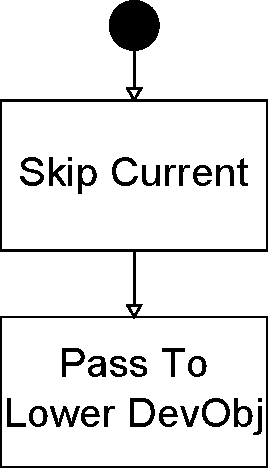
\includegraphics[width=0.2\linewidth]{./graph/df-default}
\caption{默认分发函数}
\label{fig:df-default}
\end{figure}

\item 电源事件分发函数

电源事件分发函数图\ref{fig:df-power}

\begin{figure}[h]
\centering
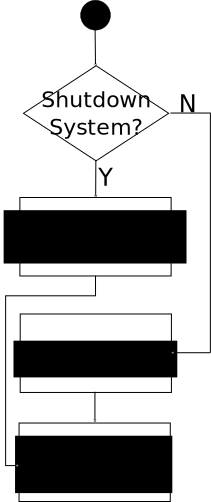
\includegraphics[width=0.3\linewidth]{./graph/df-power}
\caption{电源事件分发函数}
\label{fig:df-power}
\end{figure}

\item IOCTL分发函数

IOCTL分发函数图\ref{fig:df-ioctl}

\begin{figure}[h]
\centering
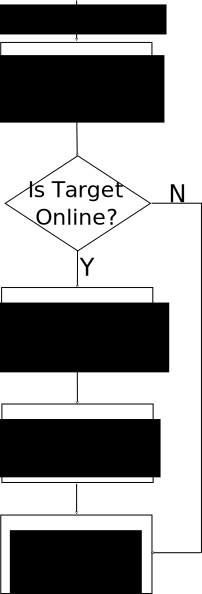
\includegraphics[width=0.3\linewidth]{./graph/df-ioctl}
\caption{IOCTL分发函数}
\label{fig:df-ioctl}
\end{figure}

\item PnP事件分发函数

PnP事件分发函数图\ref{fig:df-pnp}

\begin{figure}[h]
\centering
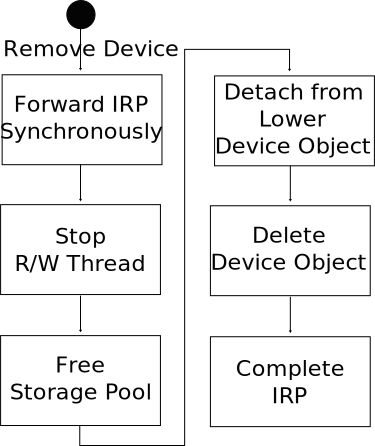
\includegraphics[width=0.4\linewidth]{./graph/df-pnp}
\caption{PnP事件分发函数}
\label{fig:df-pnp}
\end{figure}

\item 读写分发函数

读写分发函数图\ref{fig:df-rw}

\begin{figure}[h]
\centering
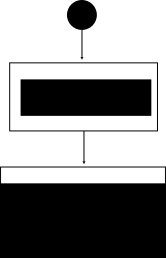
\includegraphics[width=0.2\linewidth]{./graph/df-rw}
\caption{读写分发函数}
\label{fig:df-rw}
\end{figure}

\end{enumerate}

%% ----------------------------------------------------------------------

\section{用户配置工具}
\label{sec:config_utility}

系统提供了命令行的用户配置工具,在用户层和内核层的驱动程序进行交互。通过驱动设备对象提供的IOCTL命令,来完成两个方面的功能:
\begin{enumerate}
\item 配置缓存系统的运行状态。包括启动、停止和设置作为缓存的卷。
\item 获得缓存系统的统计数据。获得IO统计信息,如读写次数和命中率。
\end{enumerate}

配置工具启动后,依据用户输入的命令完成相应操作。工具提供如下几种种命令:

\begin{itemize}
\item start
\\描述:为某个指定的HDD存储卷开启SSD缓存。
\\使用:start  [disk\_number]  [volume\_number]
\\IOCTL:IOCTL\_DF\_START

\item stop
\\描述:停止某个HDD存储卷上的SSD缓存。
\\使用:stop  [disk\_number]  [volume\_number]
\\IOCTL:IOCTL\_DF\_STOP

\item stat
\\描述:获取某个存储卷的统计数据。包括读、写操作次数,缓存命中率以及使用情况。
\\使用:stat  [disk\_number]  [volume\_number]
\\IOCTL:IOCTL\_DF\_GET\_STAT

\item clear
\\描述:清除某个存储卷的统计数据。
\\使用:clear  [disk\_number]  [volume\_number]
\\IOCTL:IOCTL\_DF\_CLEAR\_STAT

\item quite
\\描述:设置驱动程序不向内核日志输出任何日志信息。
\\使用:quite
\\IOCTL:IOCTL\_DF\_QUIET

\item verbose
\\描述:开启驱动程序的向内核日志的所有日志信息输出。
\\使用:verbose
\\IOCTL:IOCTL\_DF\_VERBOSE

\item verify
\\描述:开启或关闭SSD缓存池内数据和HDD数据的一致性验证,默认是关闭的,开启对性能影响明显,只做调试使用。
\\使用:verify
\\IOCTL:IOCTL\_DF\_VERIFY

\item q
\\描述:退出用户配置工具。
\\使用:q
\end{itemize}

%% ----------------------------------------------------------------------
%%% END OF FILE 
%% ----------------------------------------------------------------------